\section{Block Level Description} \label{sec:block_level}
Much of the block level descriptions can be seen in the high level report, but the transistor view of the leaf-cells will be described in this chapter. To find good sizes for our gates we used a very simple sizing strategy. Start small, and if the signal is to weak to drive the components, we just size it up and if necessary, make a buffer for it. The transistor schematic of the basic blocks like AND, OR, DFF etc. are simple enough that we will not include any description for them. \\

In Fig. \ref{top} an updated block diagram of the complete system can be seen.

\begin{figure}[H]
\centering
\captionsetup{justification=centering}
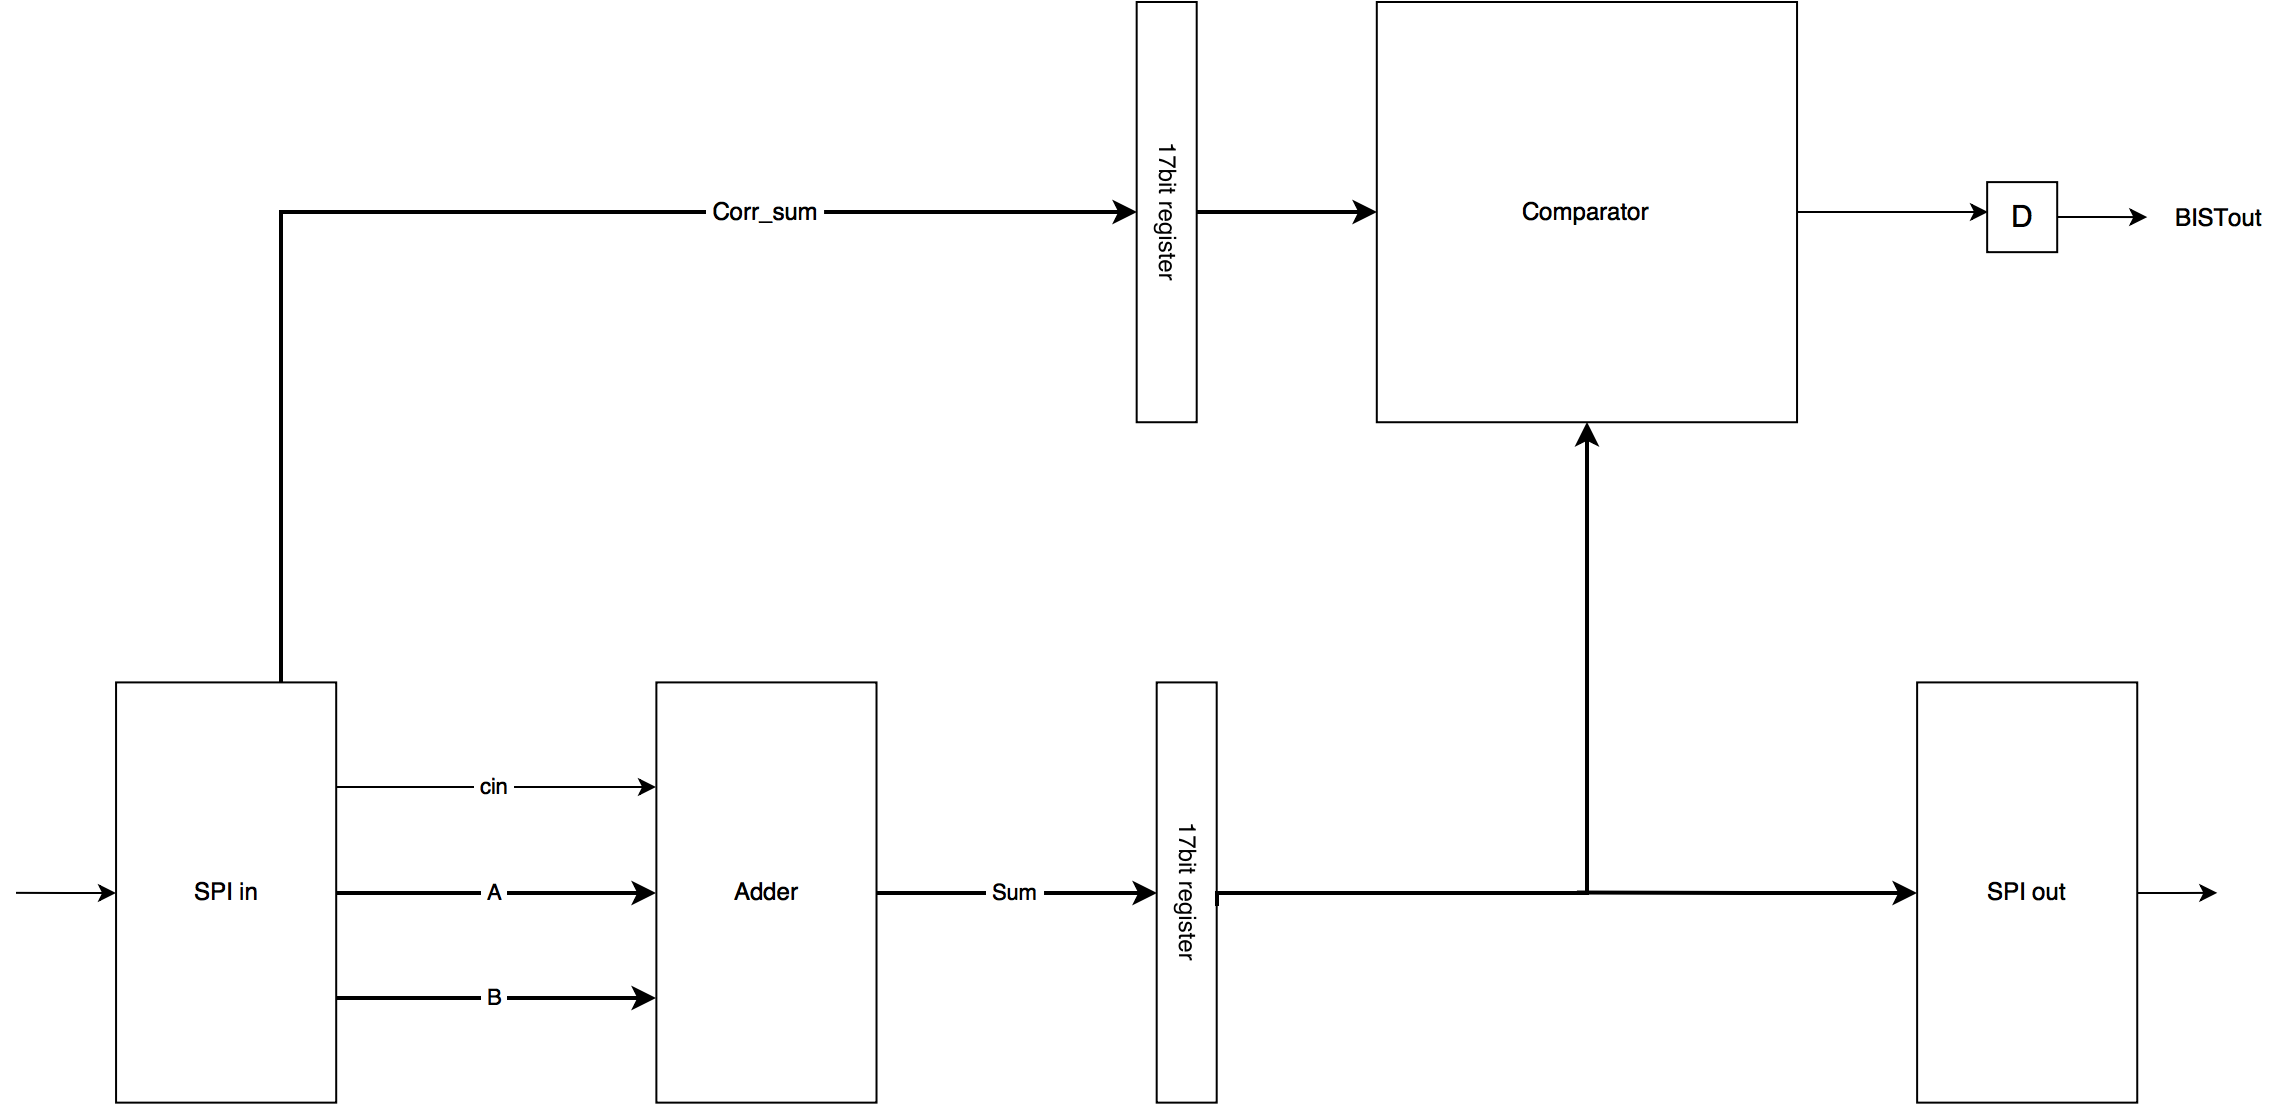
\includegraphics[scale=0.35]{../figures/top_level.png}
\caption{Top level block diagram.}
\label{top}
\end{figure}

The updated diagram contains additional registers for synchronizing the signal before and after the comparator. This was done to provide more stable signals to the comparator and to have a more easily interpreted BISTout signal. The drawback is that the BISTout signal is available two clock cycles after the addition took place.   